The results presented in this section have been obtained using the EUTelescope software described in section~\ref{sec:offline}.
The setup does not include any additional DUT, only six $\Mimosa$ telescope planes are used and unbiased track residuals for each telescope plane are calculated.

\subsection{Data Analysis Flow}
\label{sec:datura-nodut}

After conversion from raw $\Mimosa$ data, a hot pixel search is performed excluding pixels with firing frequencies above a certain threshold from the subsequent analysis.
Clusters of adjacent pixels are formed and translated from two-dimensional entities on the individual telescope planes into hits in a global three-dimensional frame of reference.
For offline alignment the tracks found by the DAF processor are passed to Millepede-II to determine shift and rotation alignment constants for every telescope plane.

%Finally the unbiased residual distributions for every telescope plane are calculated from the precisely aligned telescope hits.
In a separate iteration for every telescope plane a track fit is performed using the precisely aligned telescope hits, excluding the plane under investigation.
The tracks are extrapolated to the plane under investigation, and the residual distance between track extrapolation and plane hits as well as its tracking efficiency are calculated.

\subsection{Geometry and multiple scattering}
\label{sec:multiplescattering}
%The telescope performance has been validated at CERN (120\,GeV pions) and DESY (1 to 6\,GeV positrons). 
%In order to get realistic data description at DESY beam energies all scattering material between sensitive planes has to be taken into account. 
%The precision of the track prediction at the DUT (plane \#3) based on five other telescope planes is shown in Figure\,\ref{fig:resolution}. 
%The combination of the thickness of the telescope planes ($\unit{50}{\upmu\meter}$) with their hit position precision ($\sim\unit{3.5}{\upmu\meter}$)
% when minimising the distances to the Detector Under Test (DUT), 
% allows to sustain track pointing precision below $\unit{3}{\upmu\meter}$ for all electron (positron) energies above 2\,GeV and distance to the DUT shorter then 20\,mm (Figure\,\ref{fig:resolution}).
%More stuff:

% (comment hjansen: actually pointing resolution! comment te: pointing only in space :) )
The figure of merit for beam telescopes is their resolution, as this defines the precision with which each particle trajectory can be measured. 
%The timing resolution is largely dependent on the readout speed of the used sensors, their buffer sizes and the data acquisition system. 
Spatial resolution depends on the individual intrinsic sensor resolution, the number of measurements for each trajectory and their position, as well as the multiple scattering of the beam particles.
The expression

\begin{equation}
\label{eq:telescoperesolutionequation}
\sigma_{\textrm{meas}}^2 = \sigma_{\textrm{DUT}}^2 + \sigma_{\textrm{Tel}}^2 +
\sigma_{\textrm{MS}}^2
\end{equation}

\noindent shows the contributing terms to be considered~\cite{ref:eudetreport200902}. 
The measured residual width on a DUT sensor plane is expressed by $\sigma_{\textrm{meas}}$, $\sigma_{\textrm{DUT}}$ is the intrinsic resolution of the DUT itself,
 $\sigma_{\textrm{Tel}}$ is the resolution of the telescope and $\sigma_{\textrm{MS}}$ represents the contribution from multiple scattering.
In the following, all terms are discussed.
The resolution of a telescope $\sigma_{\textrm{Tel}}$ can be expressed by

\begin{equation}
\label{eq:telescopepointing}
\sigma_{\textrm{Tel}}^2 = k \cdot \sigmai^2
\end{equation}

\noindent with the geometric scaling factor $k$ in turn written as

\begin{equation}
k = \frac{\sum_i^N z_i^2}{N \cdot \sum_i^N z_i^2 - \left( \sum_i^N z_i \right)^2} \,,
\end{equation}

\noindent assuming all $N$ telescope planes have the same intrinsic resolution $\sigmai$. 
The distance of the $i$-th telescope plane to the DUT positioned at $z=0$ is then $z_i$ .
For a symmetric set-up with the DUT at the centre of the telescope and the up- and downstream planes equally spaced, $k$ reduces to $k = 1/N$. 

Multiple scattering is the term used to describe the deflection of a charged particle traversing any medium.
It depends on the particle energy, particle type and the radiation length of the matter traversed~\cite{ref:scatteringhighland}.
The angular scattering distribution is centred around $0$, with a width that can be expressed by~\cite{ref:PDG-2014}

\begin{equation}
\label{eq:multiplescattering}
\Theta_{0} = \frac{13.6\,\mega\electronvolt}{\beta c p} \cdot Z
\sqrt{\epsilon}
\cdot \left( 1 + 0.038 \ln{\left( \epsilon \right) } \right) \,,
\end{equation}

\noindent with the particle velocity $\beta c$, momentum $p$ and charge number $Z$. 
The expression $\epsilon = x \per X_0$ is the material budget, as defined in section~\ref{sec:radiationlengths}.

Equation~(\ref{eq:multiplescattering}) shows, that since the angular deflection due to multiple scattering increases with material budget, it is advantageous to use thin sensors.
This is especially important at low-energy beams, such as the DESY-II test beam, as the distortion increases towards lower energies.
As the beam particles also interact with the air, an additional contribution to the amount of multiple scattering depending on the distance between sensor planes has to be considered. 
At high-energy hadron beams, the contribution from multiple scattering can be neglected in general.

\subsection{Measurements with DATURA}

Measurements of the achievable resolution were performed in $2012$ to verify the performance of the $\Datura$ telescope, for different settings of beam momentum, sensor SNR threshold and sensor spacing~\cite{ref:thomas}.
The track residual distributions have been reconstructed as described in section~\ref{sec:datura-nodut}.
By using each telescope plane as a DUT, equation~(\ref{eq:telescoperesolutionequation}) is modified under the assumption that $\sigmai = \sigma_{\textrm{DUT}} = \sigma_{\textrm{M26}}$,
 leading to

\begin{equation}
\label{eq:telescoperesolutionequation_2}
\sigma_{\textrm{meas}}^2 = \sigma_{\textrm{M26}}^2 \cdot \left( 1 + k_5 \right) +
\sigma_{\textrm{MS}}^2\,,
\end{equation}

\begin{figure}[tb]
  \centering
  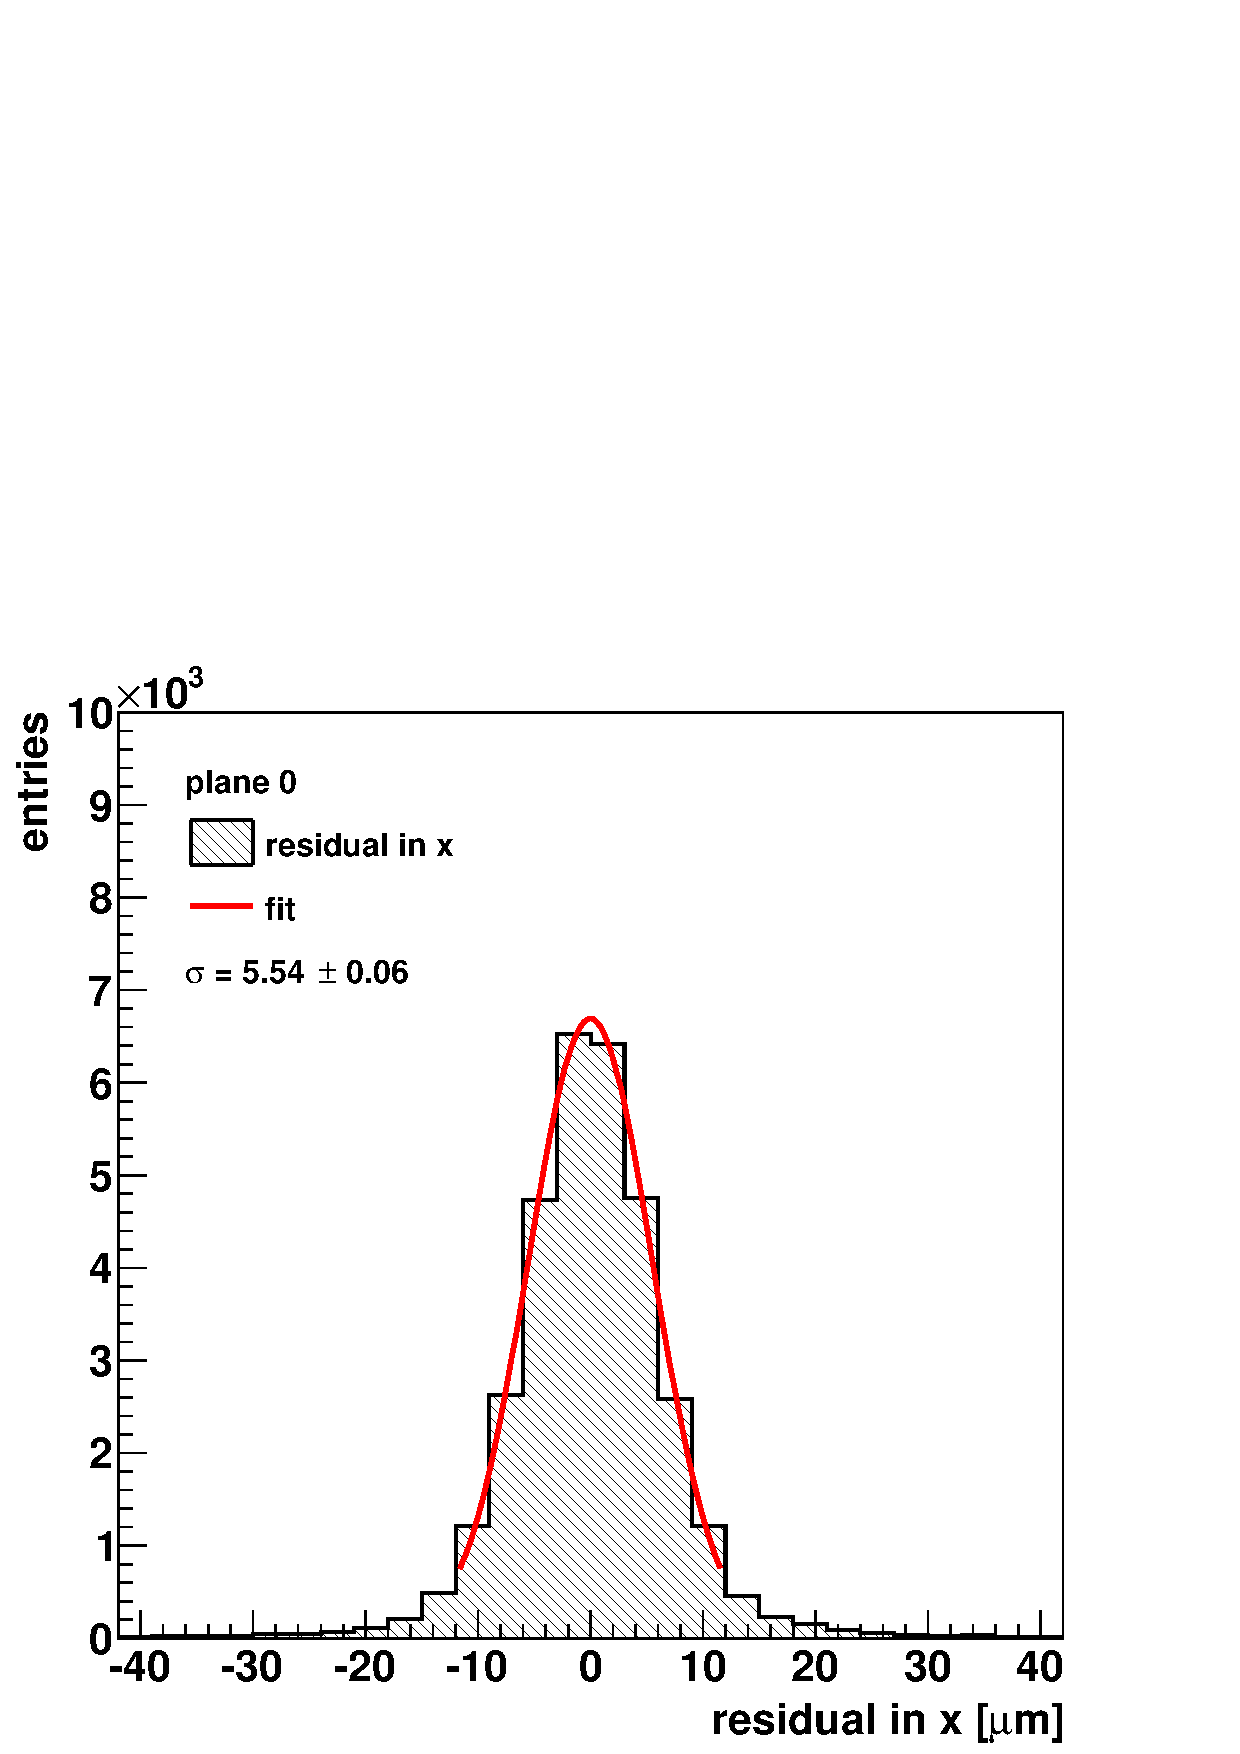
\includegraphics[width=0.45\textwidth]{figures/resis_upstream/0x.pdf}
  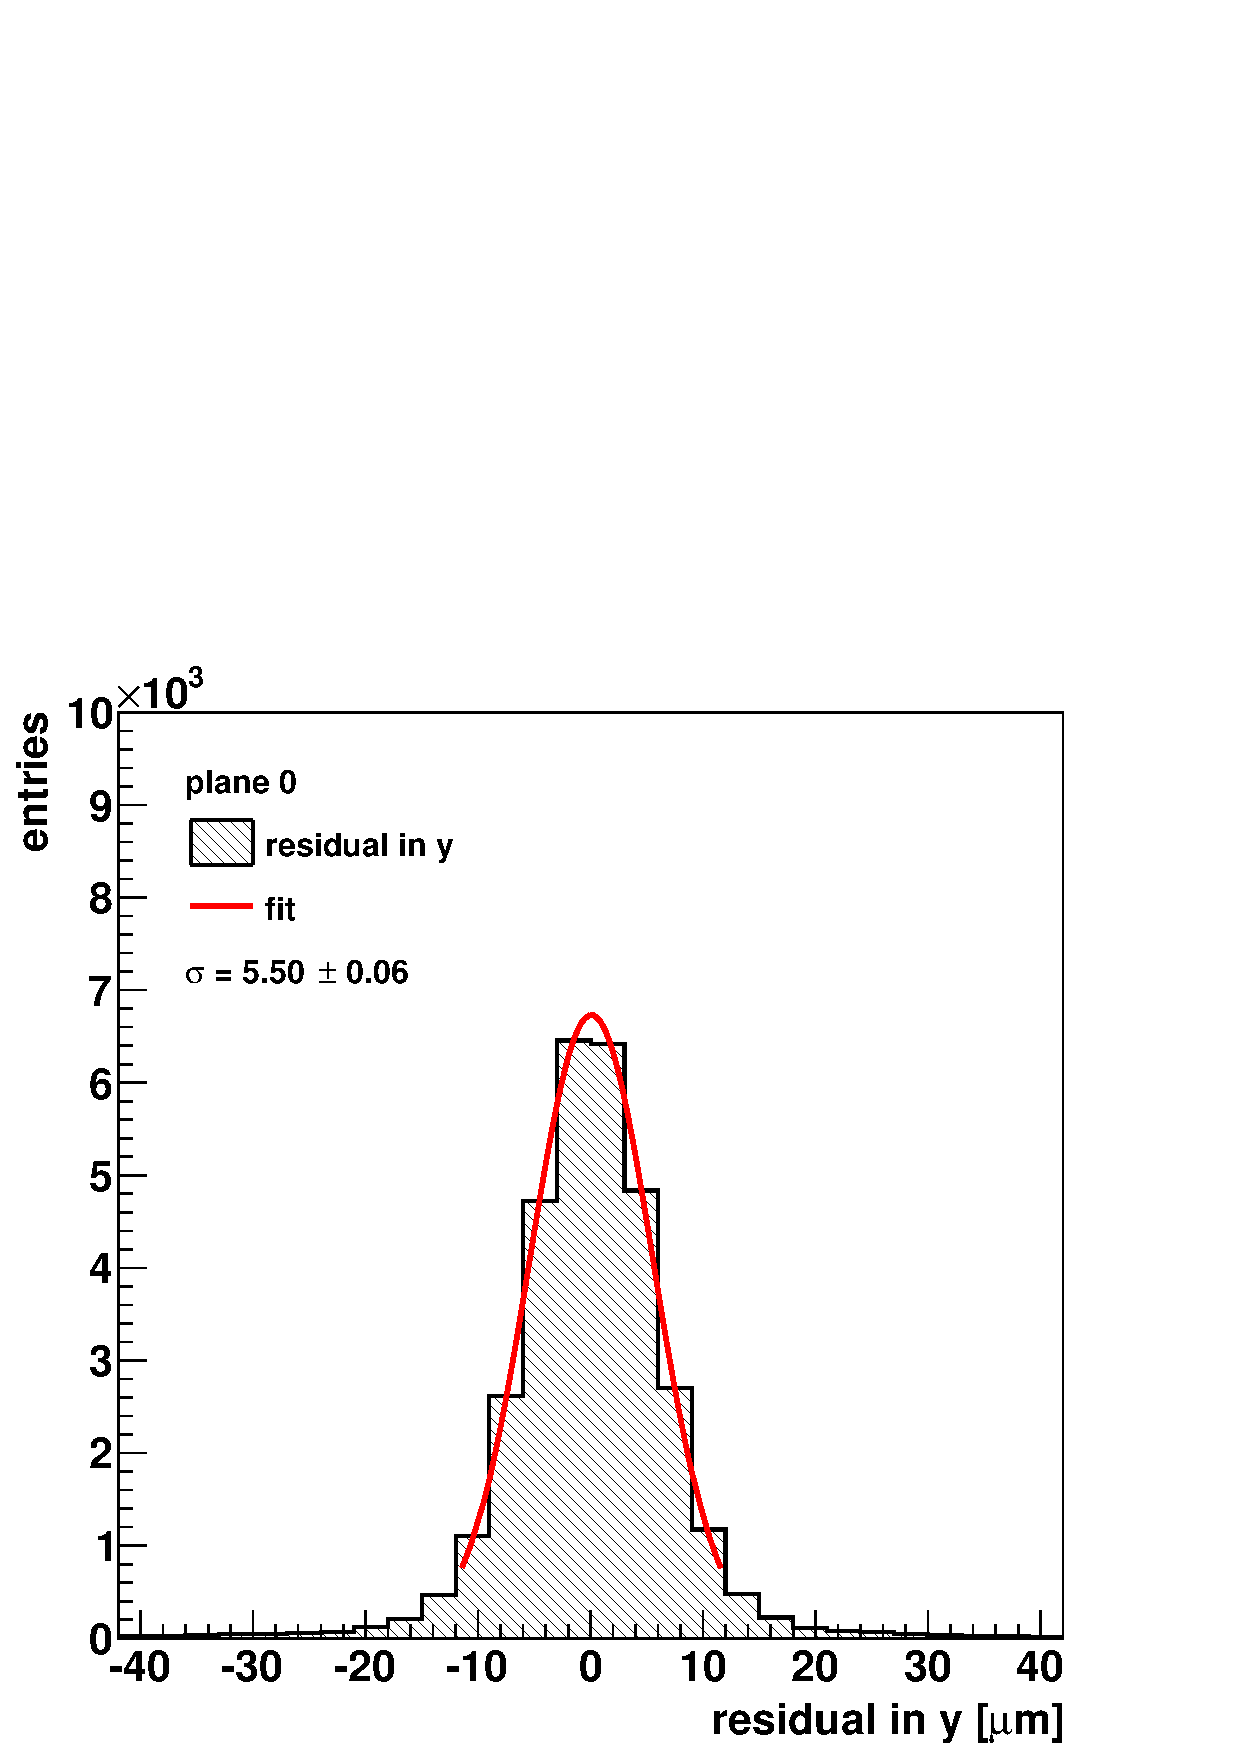
\includegraphics[width=0.45\textwidth]{figures/resis_upstream/0y.pdf}
  %\includegraphics[width=0.45\textwidth]{figures/resis_upstream/1x.pdf}
  %\includegraphics[width=0.45\textwidth]{figures/resis_upstream/1y.pdf}
  %\includegraphics[width=0.45\textwidth]{figures/resis_upstream/2x.pdf}
  %\includegraphics[width=0.45\textwidth]{figures/resis_upstream/2y.pdf}
  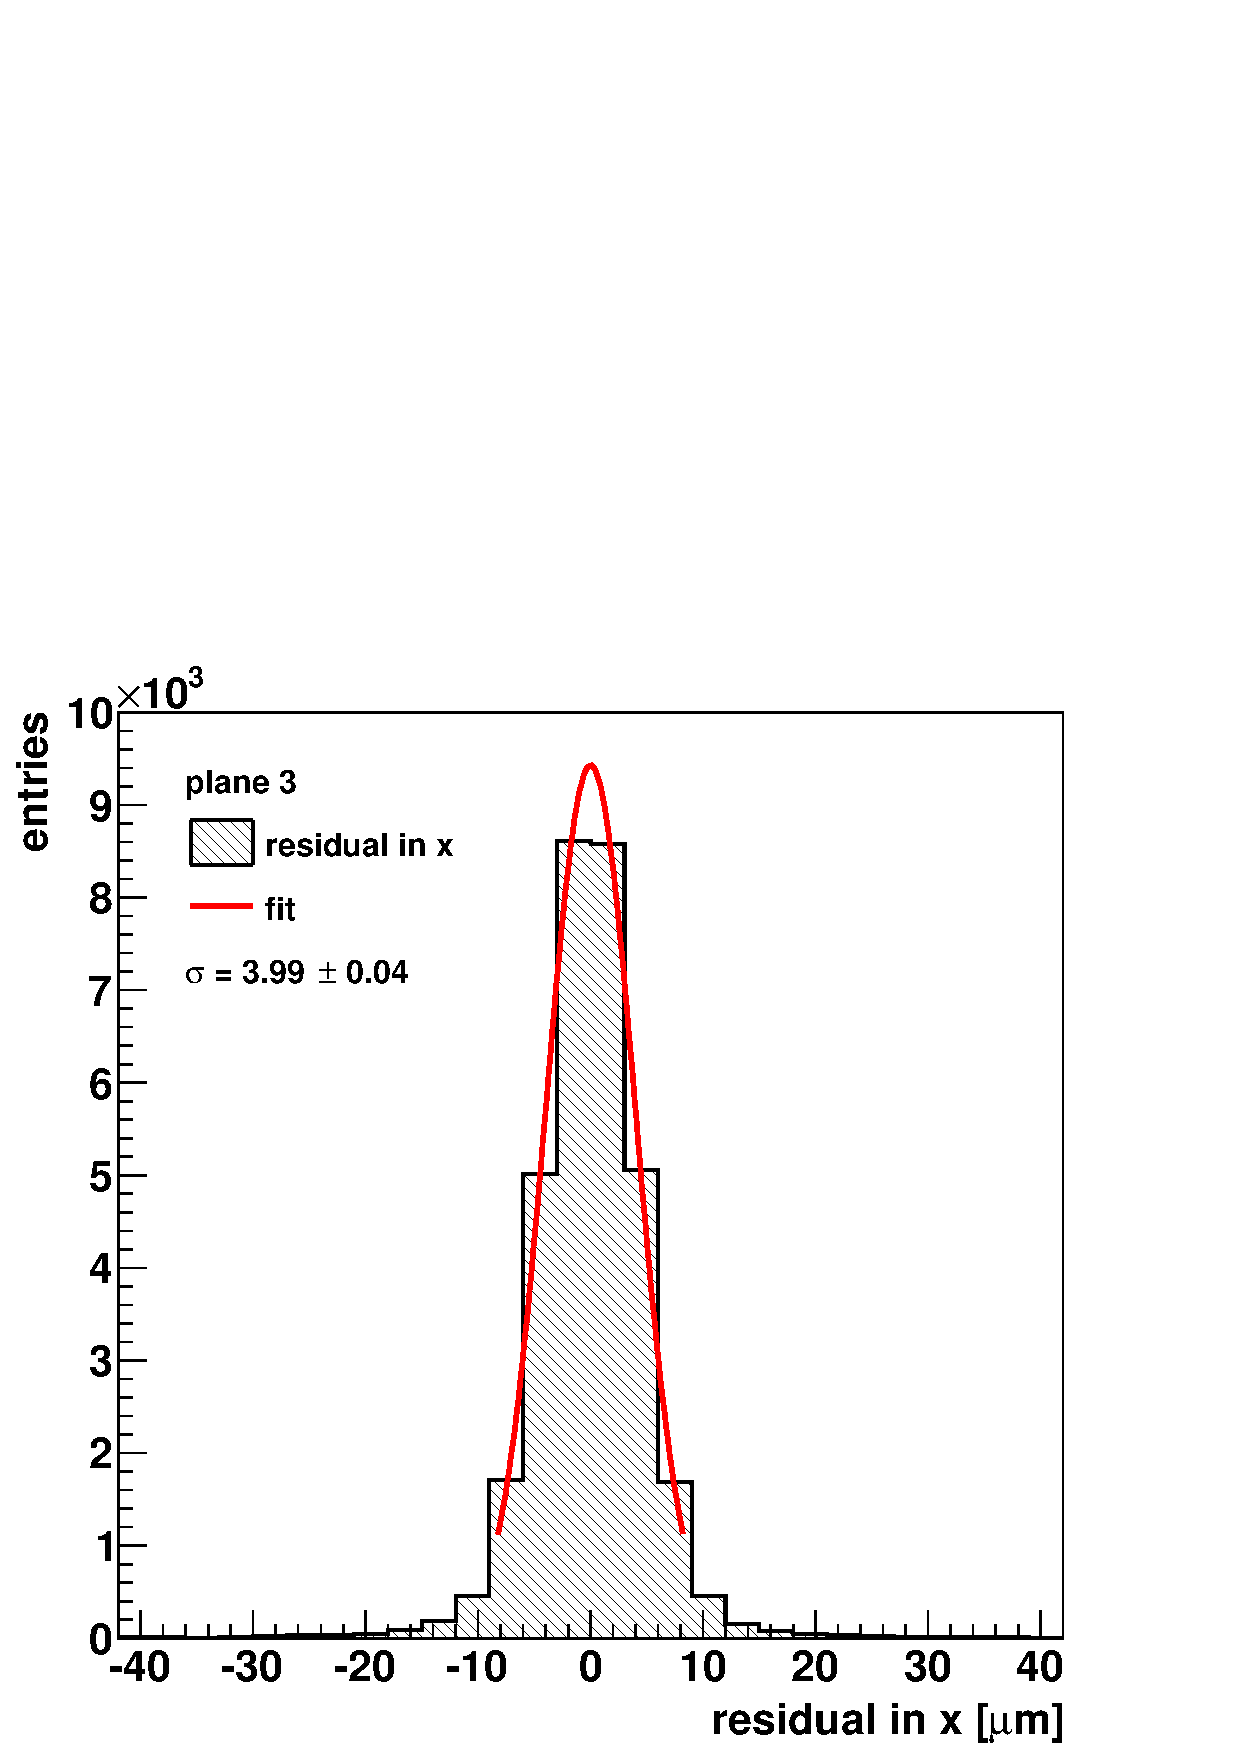
\includegraphics[width=0.45\textwidth]{figures/resis_downstream/3x.pdf}
  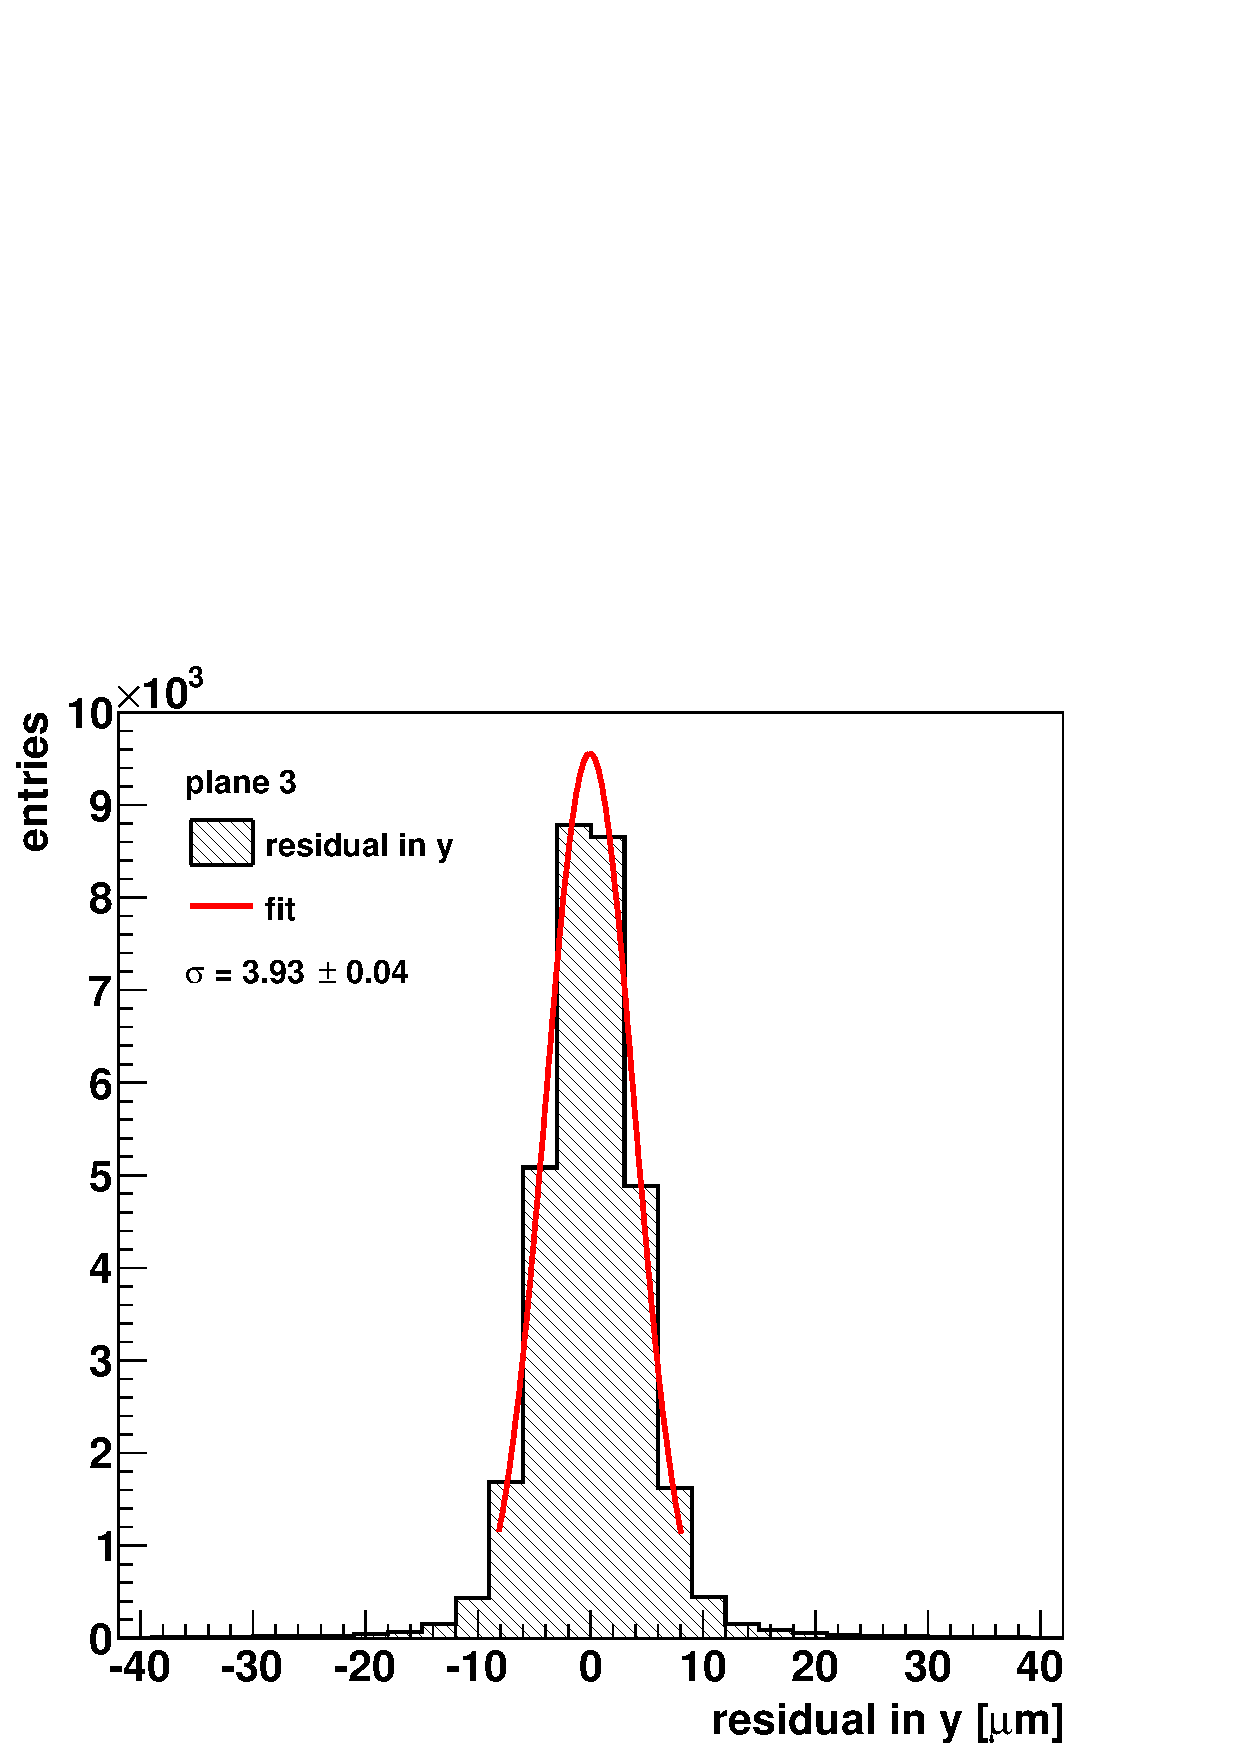
\includegraphics[width=0.45\textwidth]{figures/resis_downstream/3y.pdf}
  %\includegraphics[width=0.45\textwidth]{figures/resis_downstream/4x.pdf}
  %\includegraphics[width=0.45\textwidth]{figures/resis_downstream/4y.pdf}
  %\includegraphics[width=0.45\textwidth]{figures/resis_downstream/5x.pdf}
  %\includegraphics[width=0.45\textwidth]{figures/resis_downstream/5y.pdf}
  \caption[Residual examples to determine the $\Datura$ telescope's resolution~\cite{ref:thomas}]{Unbiased residual distributions measured with the $\Datura$ telescope.
From top to bottom: The measured residuals for planes $0$ and $3$, left for $x$ direction, right for $y$ direction.
Images from~\cite{ref:thomas}.}
  \label{fig:residualexample1}
\end{figure}

with $k_5$ the geometrical scaling factor for a telescope consisting of five planes.
Figure~\ref{fig:residualexample1} shows an example of unbiased residual distributions for a telescope sensor spacing of $20\,\milli\meter$,
 a beam momentum of $5\,\giga\electronvolt$ and a sensor SNR threshold setting of $6$.
The distributions are fitted with a Gaussian, from which the residual width $\sigma_{\textrm{meas}}$ is determined.
It is noted, that the residuals feature non-Gaussian tails, as is expected from the underlying physics of the scattering mechanism~\cite{ref:PDG-2014}. 
The measured resolution used in this work is defined as the width of a Gaussian fit on the centre $90\,\%$ of the residuals. 
The residual width for the outer plane $0$ is larger than the width obtained from plane $3$.
This is expected due to the fact that the track extrapolation to the inner sensors is done from both sides, hence is comparatively more precise than for the outer sensors, where the extrapolation can only be performed from one direction. 






% \begin{figure}[hbtp]
% \centering
% 
% \caption[Residual examples to determine the DATURA telescope's
% resolution. Downstream lever arm]{Residual examples to determine the DATURA
% telescope's resolution from the downstream lever arm. From top to bottom: The
% measured residuals for planes $3$, $4$ and $5$, left for $X$ direction, right
% for $Y$ direction. Each sensor plane was considered as a passive layer during
% the track reconstruction.}
% \label{fig:residualexample2}
% \end{figure}

By using a $\chi^{2}$ minimisation method, as shown in~\cite{ref:eudetmemo_2007_01}, which in turn is based on~\cite{ref:lutzpaper}, the intrinsic resolution of the $\Mimosa$ telescope sensors is calculated from the unbiased residual widths. For each telescope sensor dimension, the individual contribution $\Delta \chi^2_{i}$ from plane $i$ is defined as:

\begin{equation}
\label{eq:chi2contrib}
\Delta \chi^2_{i} = \left( \frac{y_{i} - p_{i}}{\sigmai} \right)^2 \Bigg|_{i \ne i_{\textrm{DUT}}} +
\left( \frac{\theta_{\textrm{i}} - \theta_{i-1}}{\Theta_{i}} \right)^2 \Bigg|_{i \ne 0,N} \,,
\end{equation}

with the telescope plane numbering beginning at $0$.
The measured hit position is denoted by $y_{i}$, the position extrapolated from the track by $p_{i}$.
The angles between the nominal beam direction and the track direction are $\theta_{i-1}$ and $\theta_{i}$.
The former is the track angle entering plane $i$, the latter the angle of the outbound track segment.
$\sigmai$ and $\Theta_{i}$ are the intrinsic resolution of sensor plane $i$ and the width of the multiple scattering distribution, according to equation~(\ref{eq:multiplescattering}), respectively.
In the following, it is assumed that $\sigmai$ does not differ between planes and is also equal for both measurement dimensions.
If the beam axis is denoted by $z$, then $\theta_i$ can be expressed as:

\begin{equation}
\theta_i = \frac{p_{i+1} - p_i}{z_{i+1} - z_i} \,.
\end{equation}


In equation~\ref{eq:chi2contrib} the first term, resulting from the hit measurement, is not included in the $\chi^2$ calculation if the plane concerned is the DUT.
Similar, for the first and last planes the second term in equation~\ref{eq:chi2contrib} is omitted, since the scattering angle can not be determined.
This results in the global $\chi^2$ expression:

\begin{equation}
\label{eq:globalchi2}
\chi^2 = \sum_{i=0}^{N} \alpha_i \left( y_i - p_i \right)^2 + \sum_{i=1}^{N-1}
\left( \frac{p_{i + 1} \beta_i + p_{i-1} \beta_{i-1} - p_i \left( \beta_i + \beta_{i-1} \right)}{\Theta_i} \right)^2 \,,
\end{equation}

with coefficients $\alpha_i$ and $\beta_i$ defined as~\cite{ref:eudetmemo_2007_01}:

\begin{equation}
\begin{aligned}
\alpha_i &= \left\{
  \begin{array}{l l}
    \sigma_{i}^{-2} & \quad \text{for $i \neq i_{\textrm{DUT}}$}\\
    0 & \quad \text{for $i = i_{\textrm{DUT}}$}
  \end{array} \right. \\
\beta_i &= \frac{1}{z_{i + 1} - z_i} \,.
\end{aligned}
\end{equation}

The minimum of equation~\ref{eq:globalchi2} is then calculated to find the intrinsic sensor resolution $\sigma_i = \sigmai$.
The results for both a tighter plane spacing of $20\,\milli\meter$ and a wider spacing of $150\,\milli\meter$ are shown in figure~\ref{fig:smiley}.\\

In both cases, an error of $2.5\,\milli\meter$ on the plane distance $\textrm{d}z$ is assumed.
The calculated intrinsic resolution $\sigma_{\textrm{M26}} = \sigmai$ of the $\Mimosa$ sensors is \allowbreak$\left( 3.42\,\pm\, \allowbreak 0.03 \right)\,\micro\meter$ for a plane spacing of $\textrm{d}z =  20\,\milli\meter$ and $\left( 3.44\,\pm\, \allowbreak 0.03 \right)\,\micro\meter$ for $\textrm{d}z = 150\,\milli\meter$.
For both geometries, the expected resolution of $\sigmai \approx\,3.5\,\micro\meter$, according to~\cite{ref:mimosa26}, can be confirmed.
The underlying assumptions in the method presented here are:\\

\begin{itemize}

\item The multiple scattering terms described in equation~(\ref{eq:telescoperesolutionequation_2}) are calculated considering the nominal sensor thicknesses, the air between sensor planes, and a $25\,\micro\meter$
thick Kapton foil on either side of each sensor.
The particle energy initially assumed prior to minimisation is the nominal beam energy.

\item The intrinsic resolution $\sigmai$ of all sensor planes is assumed to be equal.
As the discriminator SNR thresholds are set for subframes of each plane individually, however, this is not necessarily true.
%Figure~\ref{fig:resivsenergy_thresh} shows the dependence of $\sigmai$ on the applied SNR threshold.

\end{itemize}

%\item Residual widths are calculated using straight line tracks only.
%Inclined tracks, or a deflection of tracks in planes or scattering material, are not taken into account.
%However, as shown in~\cite{ref:lutzpaper}, angular deflections are then considered for the later $\chi^2$ minimisation.

\begin{figure}[tbp]
  \centering
  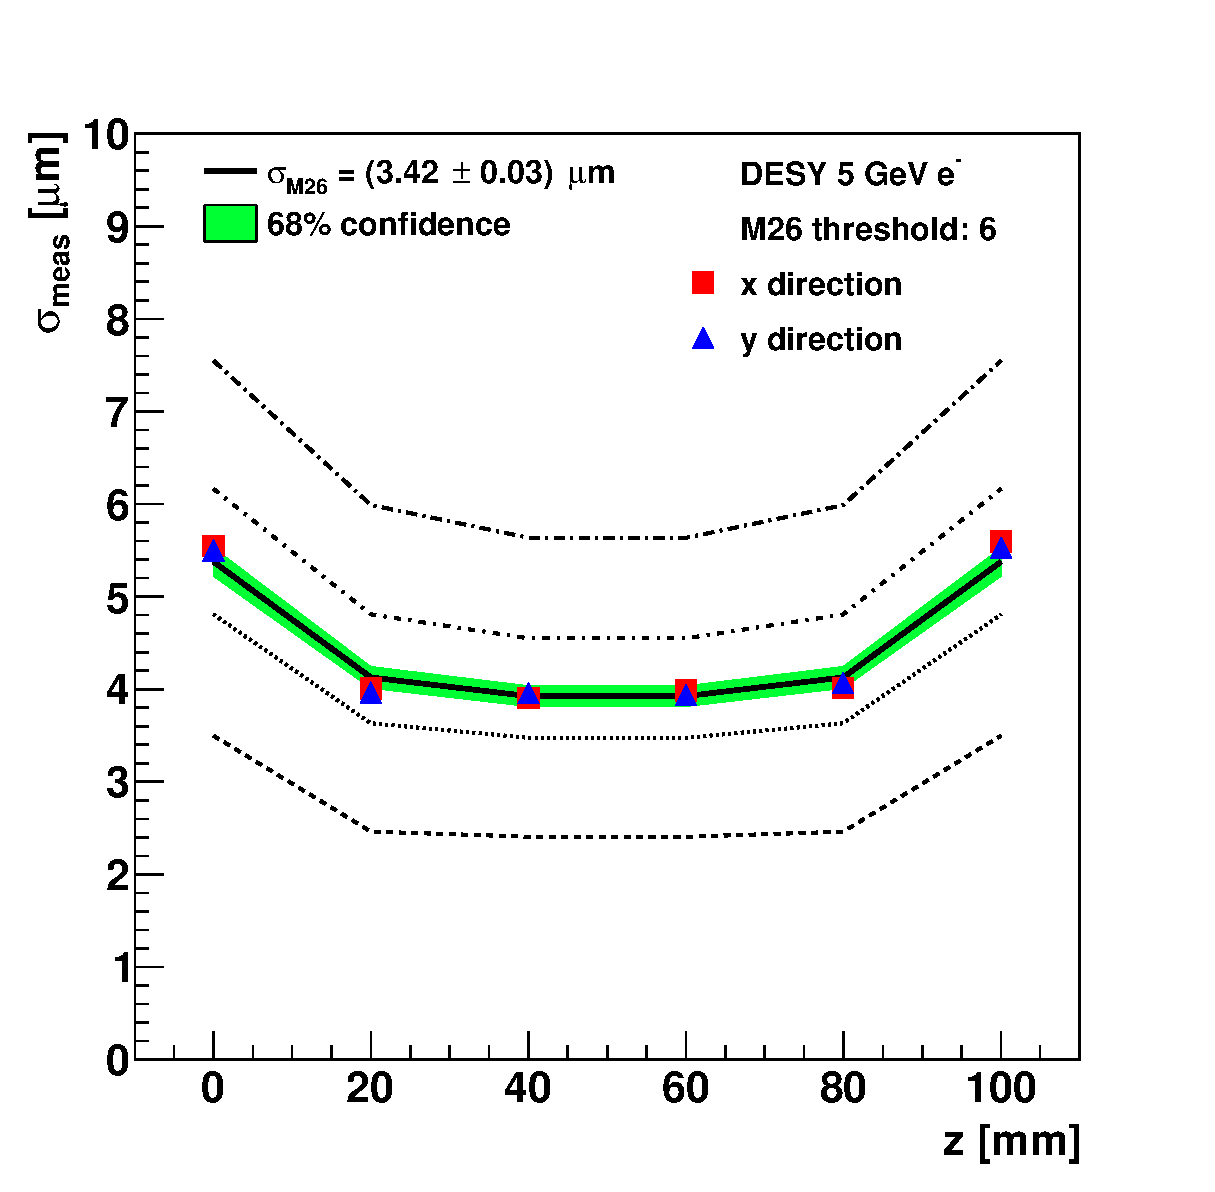
\includegraphics[width=0.49\textwidth]{figures/20} % was thin_smiley.pdf
  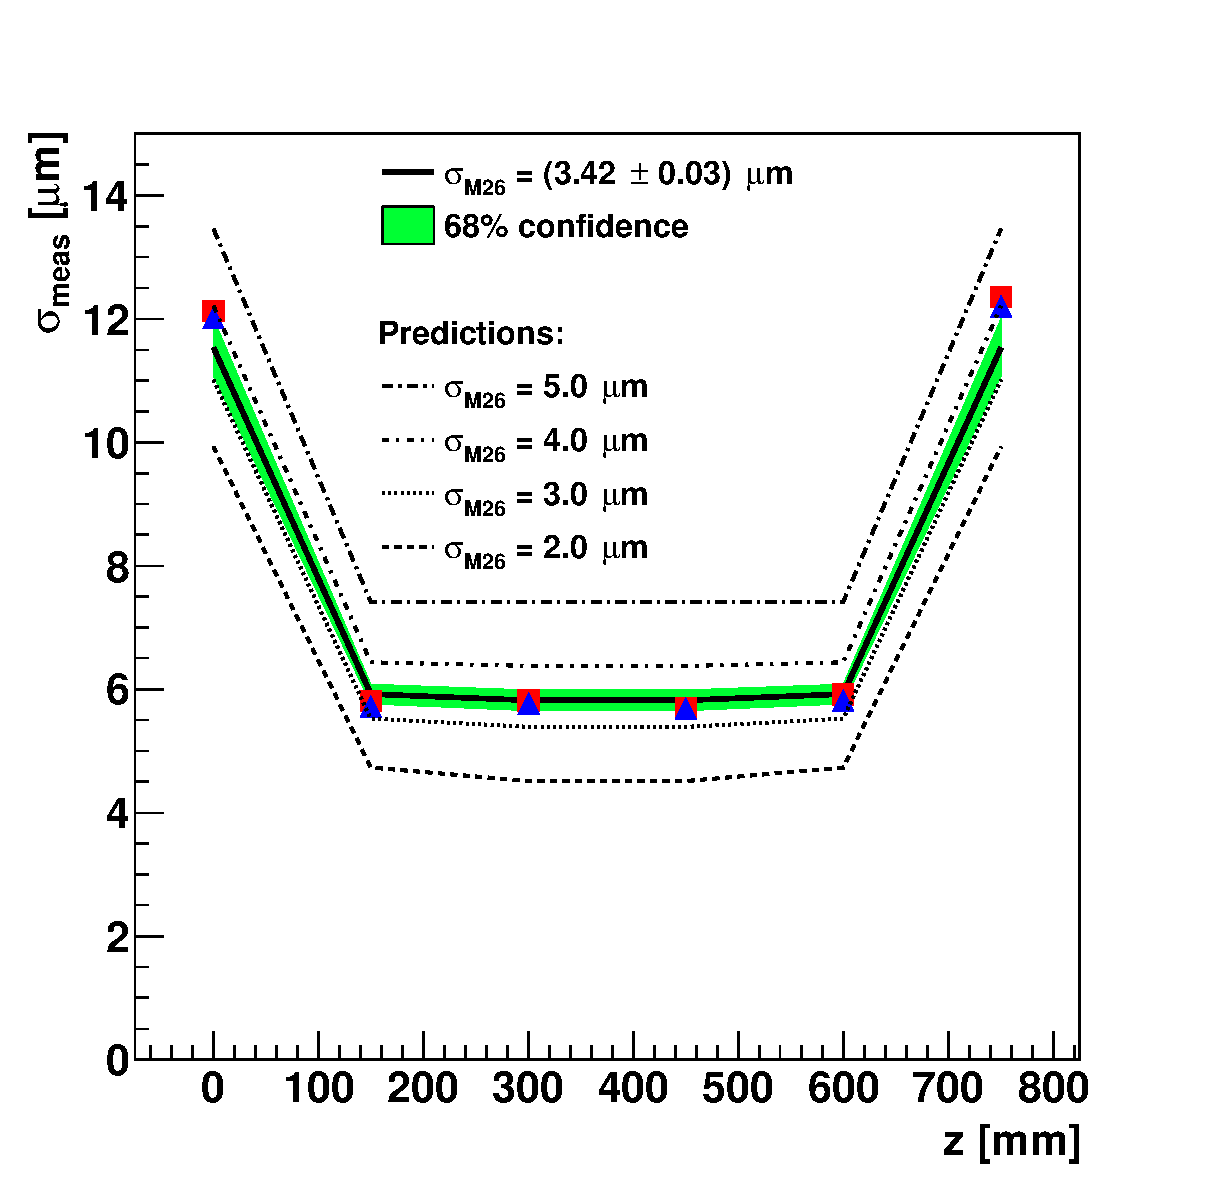
\includegraphics[width=0.49\textwidth]{figures/150} % was wide_smiley.pdf
  %\caption[Intrinsic telescope sensor resolution at $20\,\milli\meter$ and $150\,\milli\meter$ plane spacing~\cite{ref:thomas}]{Intrinsic telescope sensor resolution at $20\,\milli\meter$ (top)
  % and $150\,\milli\meter$ (bottom) plane spacing.
  \caption[The measured residual widths of each telescope plane.]{The measured residual widths of each telescope plane are shown in both the $x$ and $y$ direction for the $20\,\milli\meter$ (top)
   and $150\,\milli\meter$ (bottom) plane spacing.
  Dotted and dashed lines indicate the predicted measurements, if a different intrinsic resolution is assumed.
  The black line shows the calculated intrinsic telescope sensor resolution, the green band the measurement variance.
  For both telescope geometries, data was taken at a sensor SNR threshold setting of $6$ and with $5\,\giga\electronvolt$ electrons at DESY-II.
  Images from~\cite{ref:thomas}.}
  \label{fig:smiley}
\end{figure}

Figure~\ref{fig:resivsenergy_thresh} (A) shows the calculated intrinsic telescope sensor resolution $\sigmai$ for different beam energies and plane distances as a function of applied sensor threshold.
The minimum of $\sigmai$ is reached for a threshold setting of $6$.
The measured residual width for wider sensor spacings or lower beam energies is higher as can be seen in figure~\ref{fig:smiley}.
These effects are accounted for in equation~(\ref{eq:telescoperesolutionequation}) by the terms $\sigma_{\textrm{Tel}}^2$ and $\sigma_{\textrm{MS}}^2$.
Measurements by Behr\,\cite{ref:j.behrmeasurements} taken at $\noise\,>\,10$ show comparable results of $\sigma_{\textrm{M26}} = (4.35\,\pm\,0.10)\,\micro\meter$.\\


% Thomas: sigma tel is different from the pointing resolution.
% leave this out as to not confuse reader.
%From equation~(\ref{eq:telescopepointing}) the optimal track pointing resolution $\sigma_{\textrm{Tel}}$ of the $\Datura$ telescope without multiple scattering
% can therefore be given as $\left( 1.40 \pm 0.05 \right)\,\micro\meter$.


\begin{figure}[tbp]
  \centering
  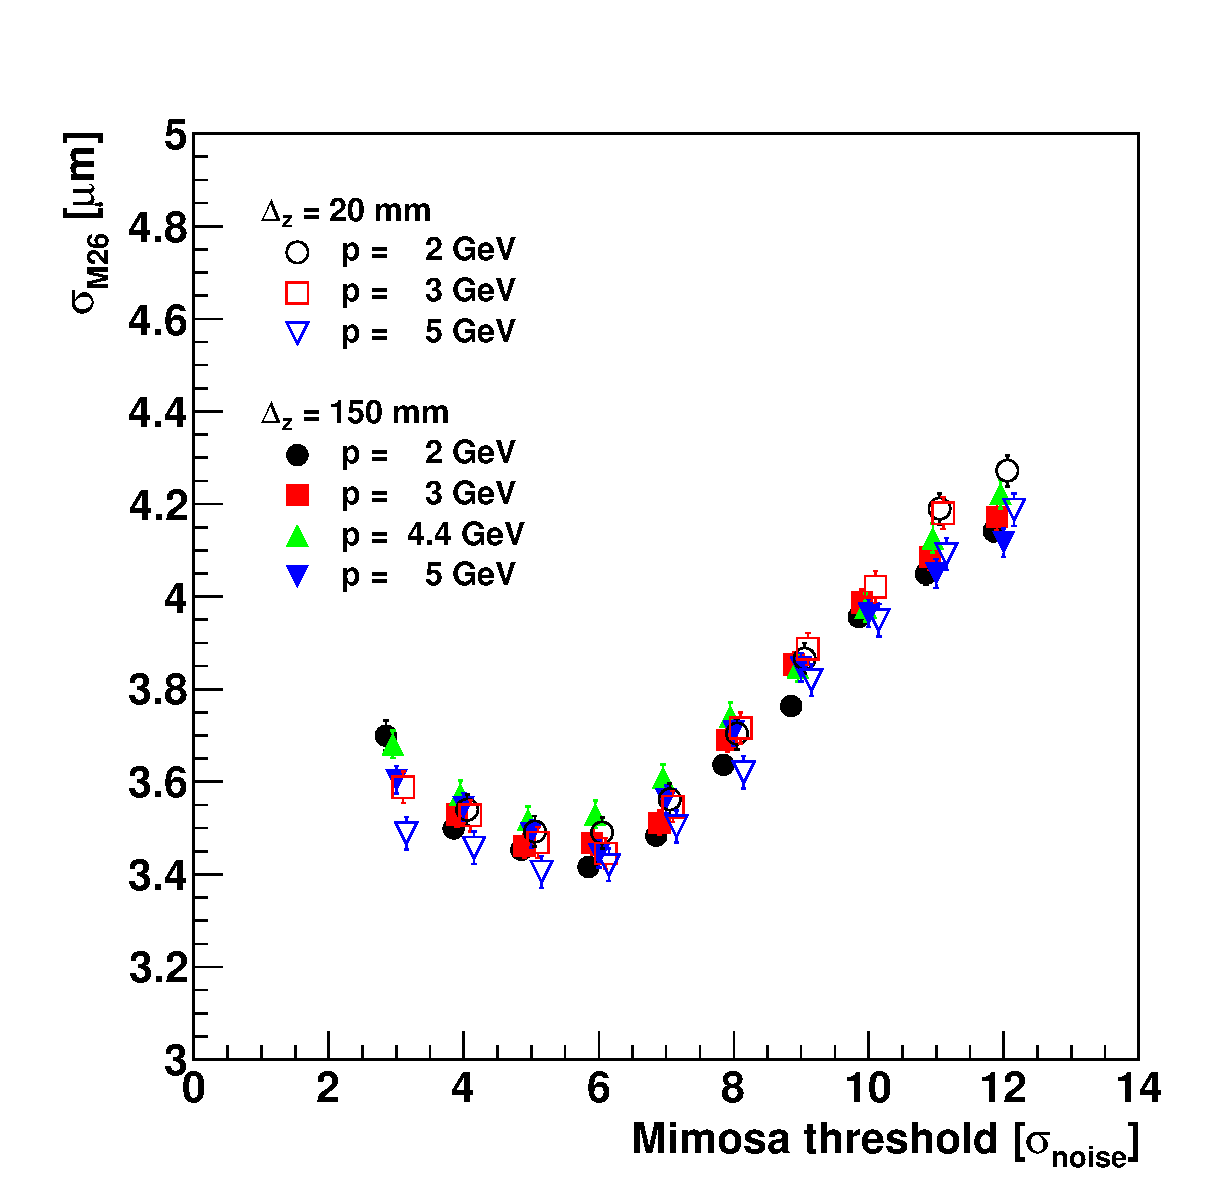
\includegraphics[width=0.49\textwidth]{figures/resi_vs_thresh}	\put(-40,170){(A)} % was resi_thresh_errors
  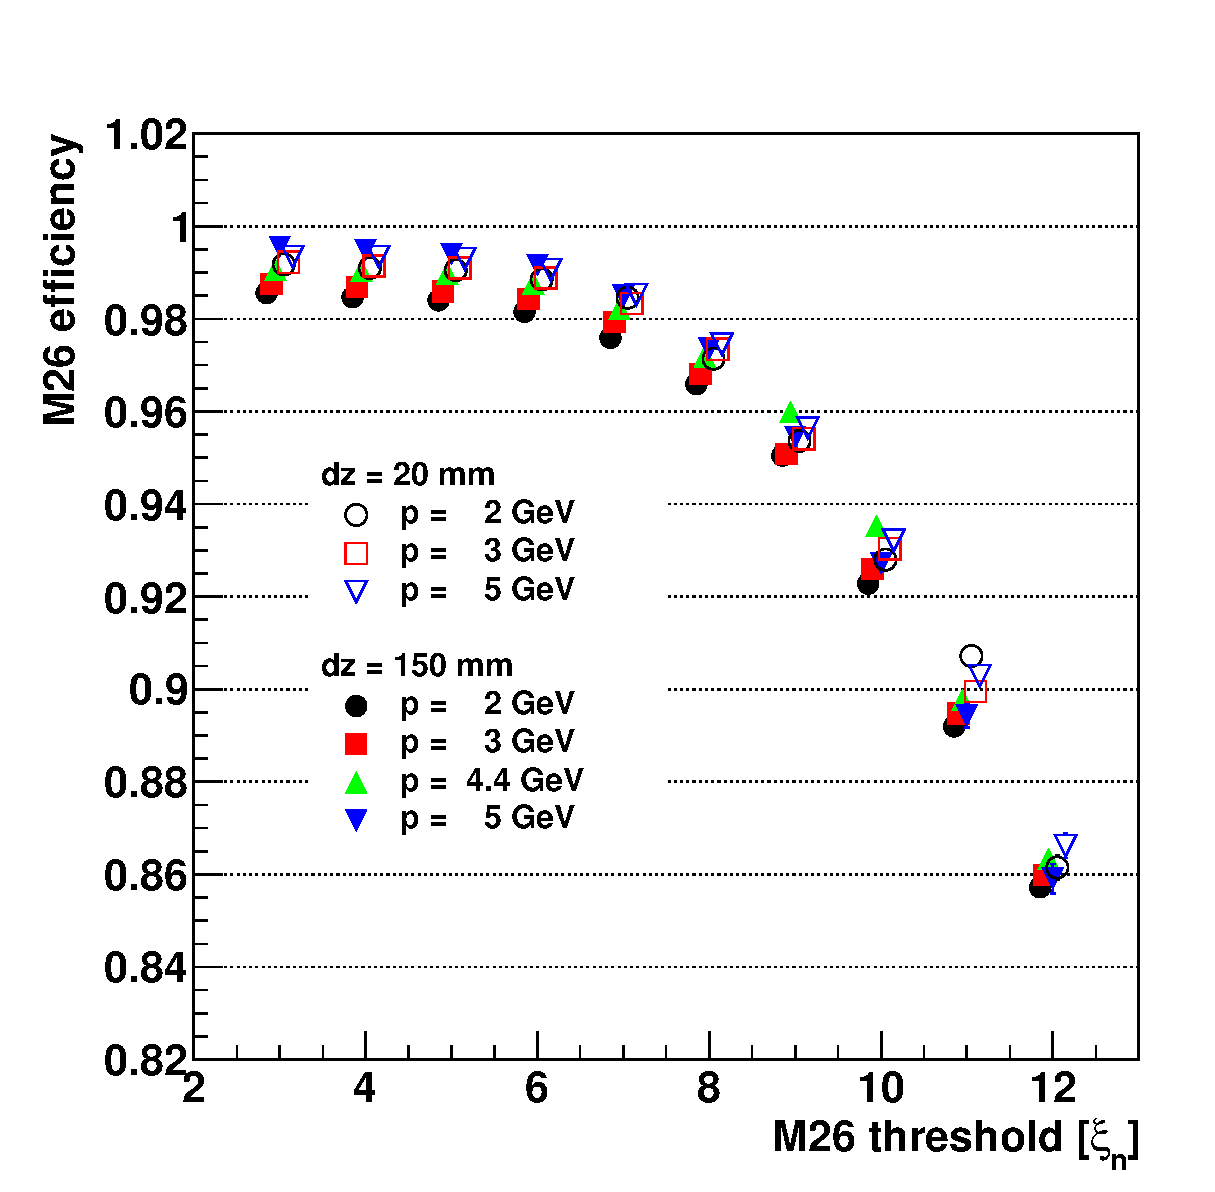
\includegraphics[width=0.49\textwidth]{figures/effi_thresh.eps}	\put(-40,170){(B)}
  \caption[Telescope intrinsic sensor resolution for different threshold settings, beam momenta and geometries~\cite{ref:thomas}]{
(A) The measured intrinsic resolution of the $\Datura$ telescope's $\Mimosa$ sensors $\sigma_{\textrm{M26}}$ for different beam momenta $p$, sensor spacing $\textrm{d}z$ and applied sensor threshold.
(B) Average efficiency of all telescope sensors in both dimensions for different beam momenta and sensor spacing vs. applied threshold.
An efficiency decline with increasing threshold can be observed.
In both images, taken from~\cite{ref:thomas}, some values are shifted on the $x$ axis for improved legibility.}
  \label{fig:resivsenergy_thresh}
\end{figure}

The threshold applied to each telescope sensor is a critical parameter for the telescope performance.
A higher threshold cuts into the signal, reducing the amount of clusters found on each plane and thus limiting the number of reconstructible tracks.
This reduces sensor efficiency.
A lower threshold allows for an increasing number of noise induced signals to be pass the zero-supression on the chip.
This leads to a broadening of the residual distributions and hence a worse resolution. 
%Figure~\ref{fig:effi} shows the efficiency distribution over a sensor plane.
The efficiency is defined as the ratio of reconstructed tracks that have at least one hit on the DUT within $100\,\micro\meter$ to the overall number of tracks.
%As maximum distance $100\,\micro\meter$ is considered.
%A noisy pixel column at $Y \approx -8\,\milli\meter$ can be observed.
%This column was masked during the converter step in the \texttt{datura-noDUT} example and subsequently is not used during the analysis. 
%\\{comment hj: datura-noDUT is jargon}\\
%Disregarding this area, an overall average efficiency over $98\,\%$ is observed.
In figure~\ref{fig:resivsenergy_thresh} (B) the efficiency dependence on the sensor threshold is shown for various beam energies and sensor spacings.
Efficiencies are averaged over all six sensor planes and both spatial coordinates, resulting in negligible statistical errors. 
In all cases, the efficiency is above $98\,\%$ up to a threshold of $7$.
With increasing threshold, the efficiency declines until an efficiency of $86\,\%$ at $\noise = 12$ is reached.
The difference between energy and plane spacings stems from multiple scattering and increased telescope resolution.

%\begin{figure}[tbp]
%  \centering
%  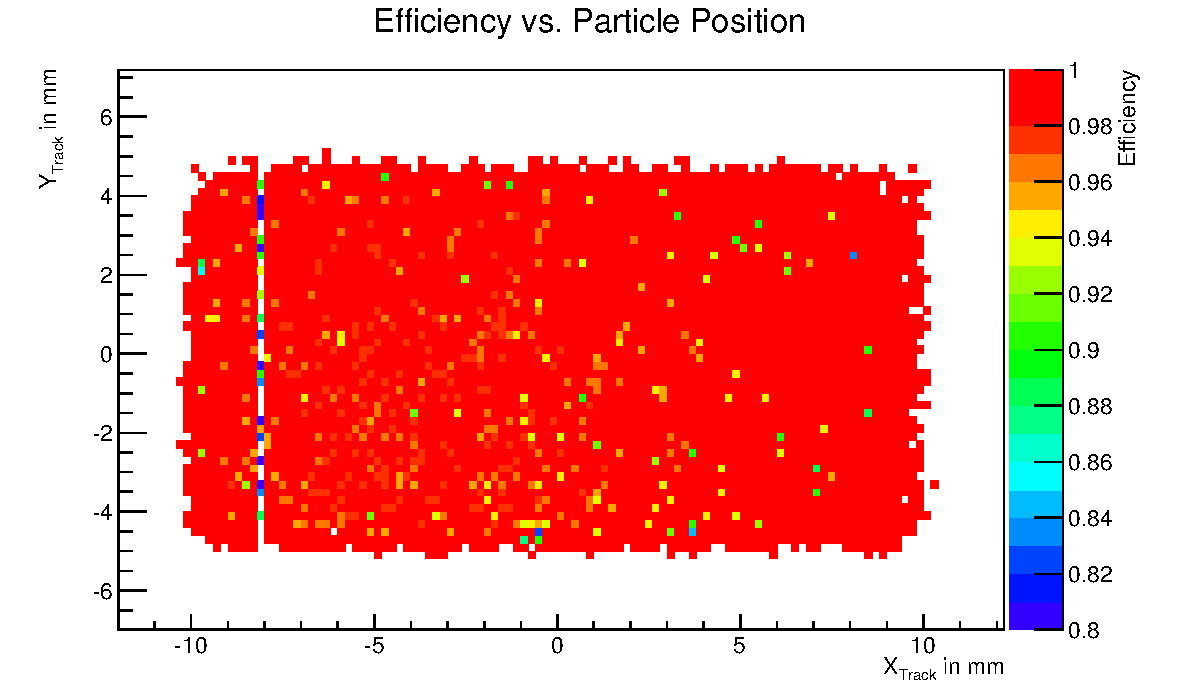
\includegraphics[width=\textwidth]{figures/plane3_effi_run37.pdf}
%  \caption[Telescope sensor efficiency~\cite{ref:thomas}]{Efficiency of telescope sensor plane $3$ at a threshold of $7$ and $5\,\giga\electronvolt$ beam momentum.
%Image from~\cite{ref:thomas}.}
%\label{fig:effi}
%\end{figure}



%\begin{figure}[tbp]
%  \centering
%  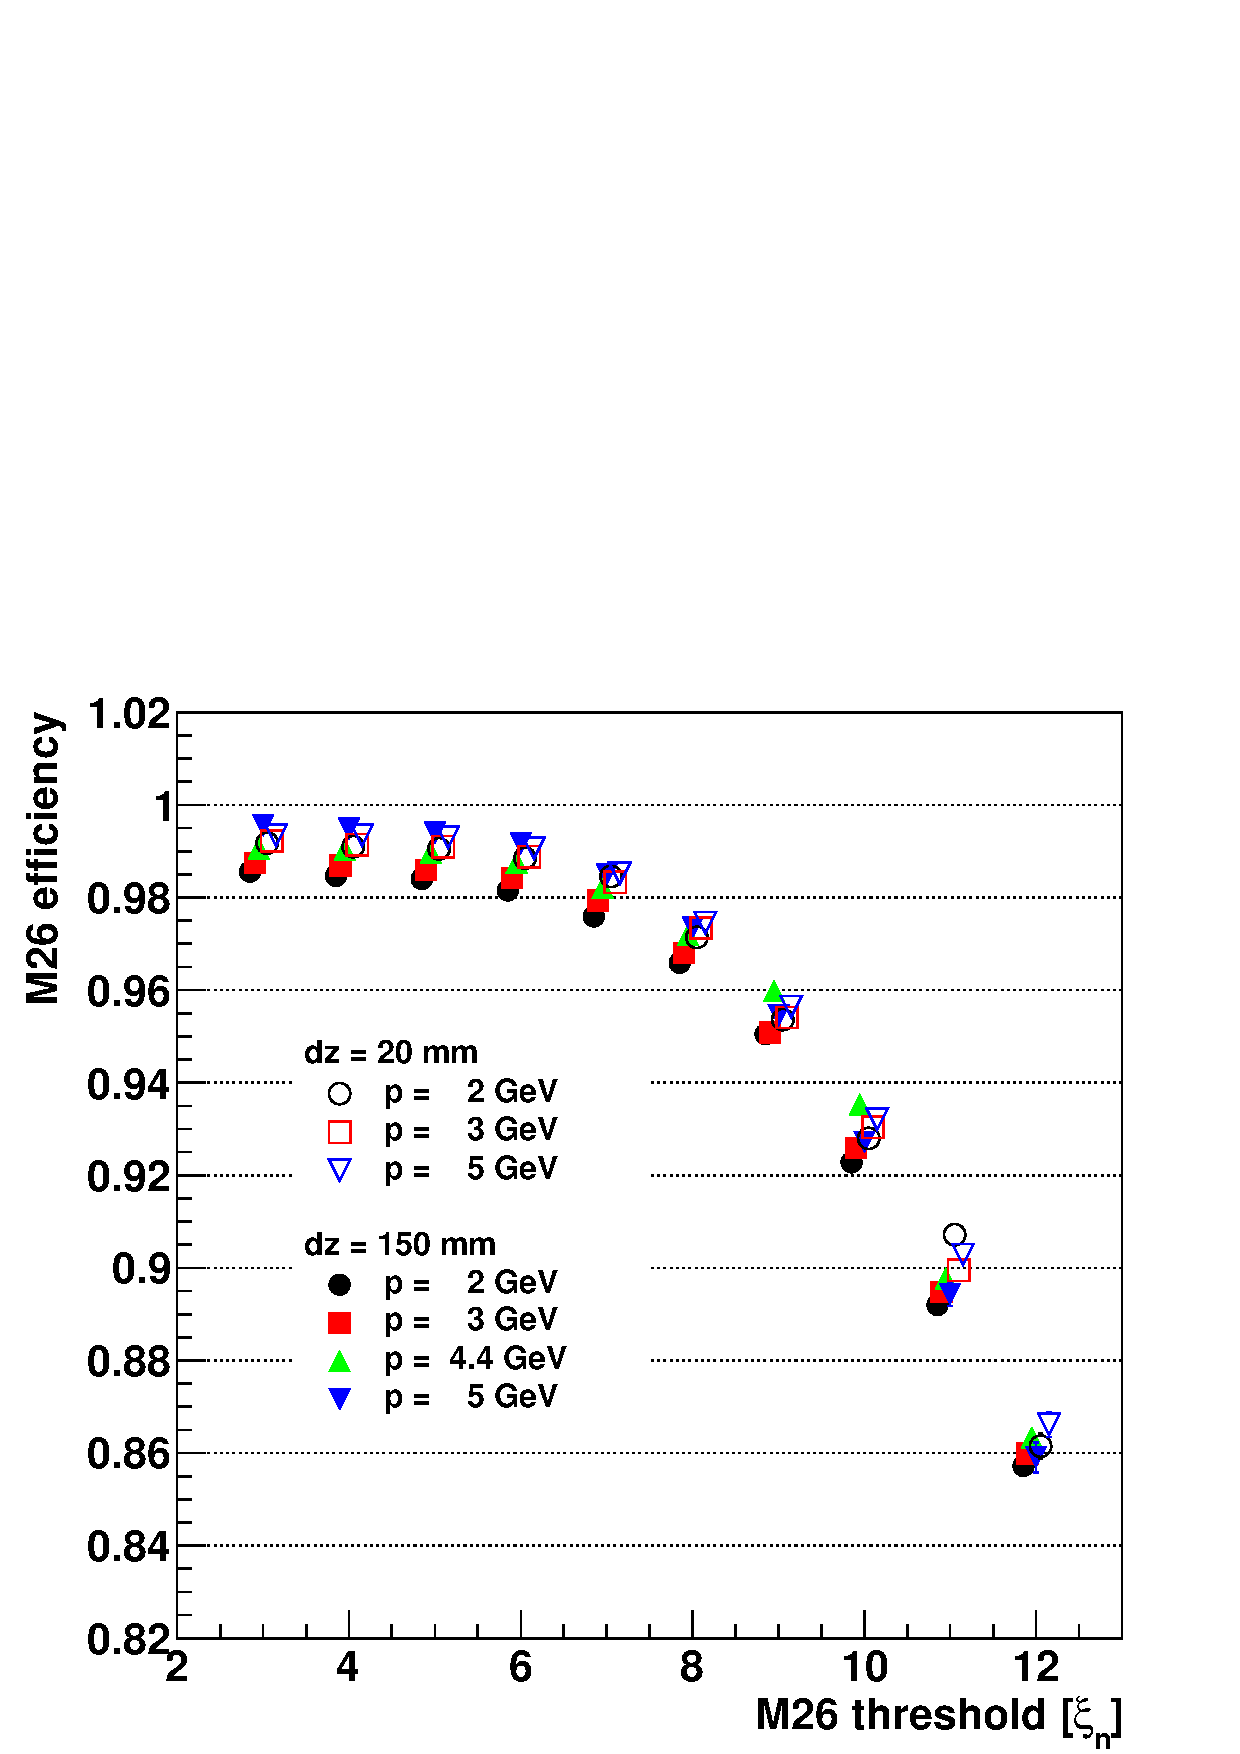
\includegraphics[width=\textwidth]{figures/effi_thresh.pdf}
%  \caption[Overall telescope sensor efficiency vs. threshold for different beam momenta and sensor spacings~\cite{ref:thomas}]{
%Average efficiency of all telescope sensors in both dimensions for different beam momenta and sensor spacing vs. applied threshold.
%An efficiency decline with increasing threshold can be observed.
%Some values are shifted on the $x$ axis for improved legibility.
%Image from~\cite{ref:thomas}.}
%\label{fig:effi_thresh}
%\end{figure}



\subsection{Resolution predictions using General Broken Lines}

With the measured intrinsic resolution at hand, and the knowledge about the amount of material of the sensor planes, predictions of the expected pointing resolution at the actual DUT position can be made. 
Therefore, it is possible to calculate a priori the optimal telescope geometry for a certain measurement set-up. 
Pointing resolutions in this section therefore therefore refer to the achievable pointing resolution using a ``symmetric six planes plus DUT'' configuration,
 cf.~figure~\ref{fig:datura_sketch}, if not stated otherwise.
Using the GBL formalism \cite{Kleinwort-2012,Blobel-2006}, the pointing resolution is analytically calculated at desired points of interest along the particle trajectory. 
Assuming $\epsmimo = 0.00071$, the pointing resolution at the DUT for four different DUT material budgets $\epsdut$ is plotted as a function of the spacing $\dzdut$
 for two fixed values of $\dz = 20\,\milli\meter$ and $50\,\milli\meter$ in figure~\ref{fig:CalcResos_dzdut}. 
Plots are provided for DESY\,II beam energies (left) and SPS energies (right). 
All plotted resolution functions are monotonically increasing with increasing $\dzdut$. 
Therefore, the optimal position of the $\Mimosa$ planes nearest to the DUT need to always be installed as close to the DUT as possible in order to achieve the best possible resolution. 
Also from figure~\ref{fig:CalcResos_dzdut} it can be seen, that the optimal plane spacing $\dz$ depends on the actual material budget of the DUT and the actual space needed for the DUT, hence $\dzdut$.
E.g.~for a DUT with a material budget of $\epsdut = 0.001$ (black and red solid line) at 5\,GeV/$\cspeed$, a narrow configuration is preferred for $\dzdut < 70\,\milli\meter$,
 but a wide configuration for $\dzdut > 70\,\milli\meter$.
The position of the intersection depends on the material budget of the DUT and decreases with increasing material budget. 
In a wide configuration, the pointing resolution is limited to about $2.3\,\upmu\meter$, whereas in a narrow configuration a pointing resolution around $2.0\,\upmu\meter$ is achievable for thin DUTs.
At SPS energies, the resolution functions for the wide and the narrow configuration do not cross, with the narrow configuration being slightly better than the wide one.
However, the difference e.g.~for $\epsdut = 0.01$ is less than $300\,\nano\meter$ for $\dzdut = 100\,\milli\meter$.

\begin{figure}[tbp]
  \centering
  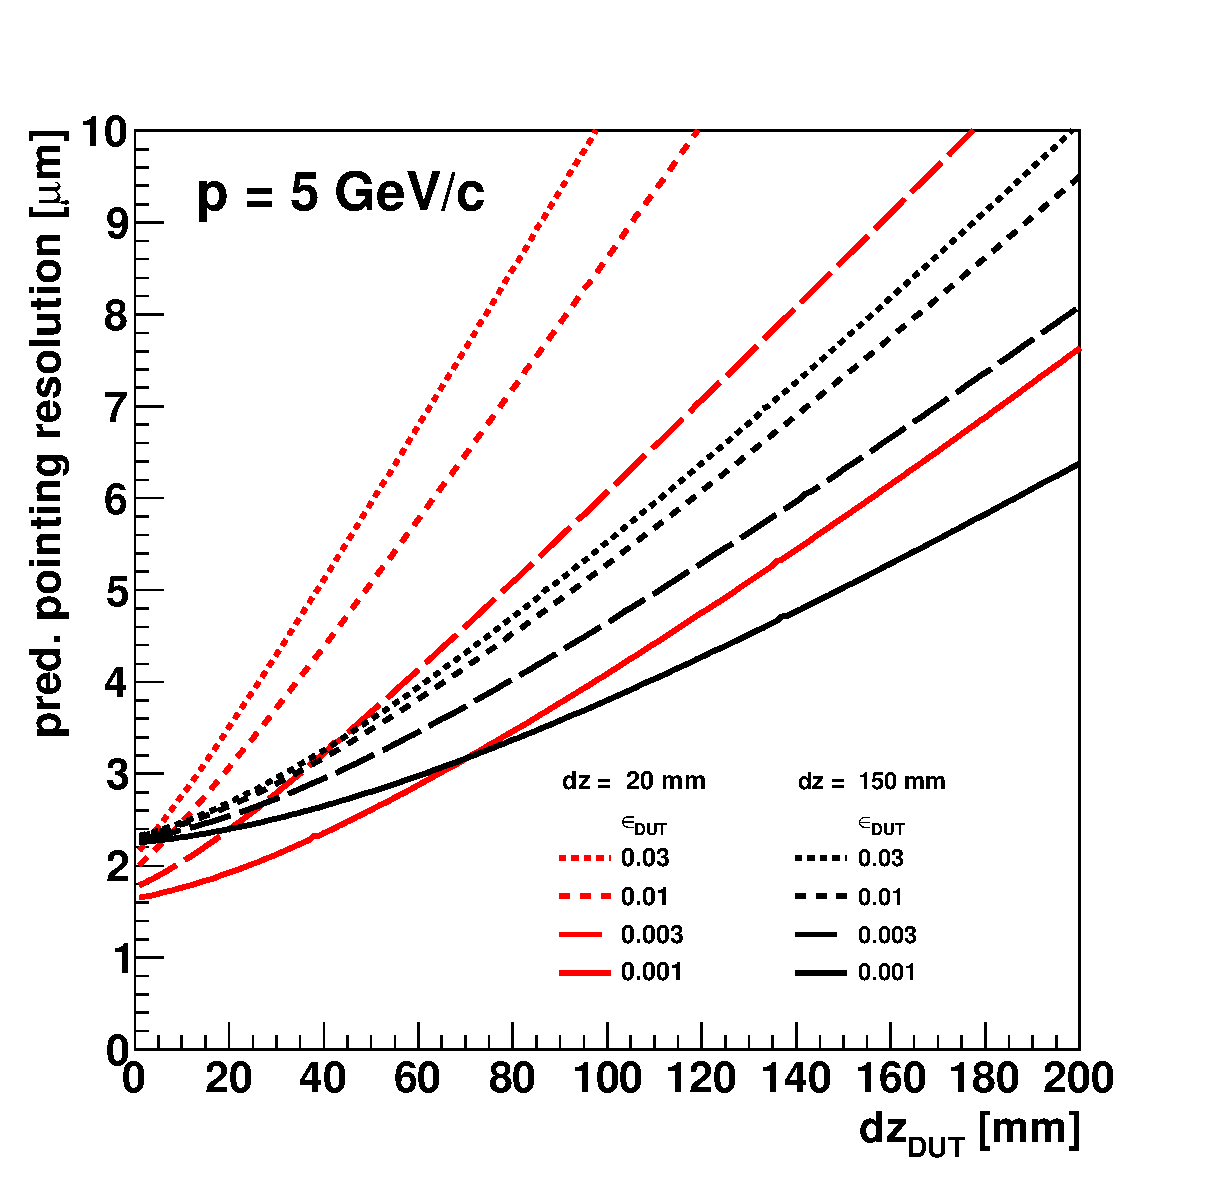
\includegraphics[width=0.49\textwidth]{figures/CalcResoVsDzdut_Desy_2}
  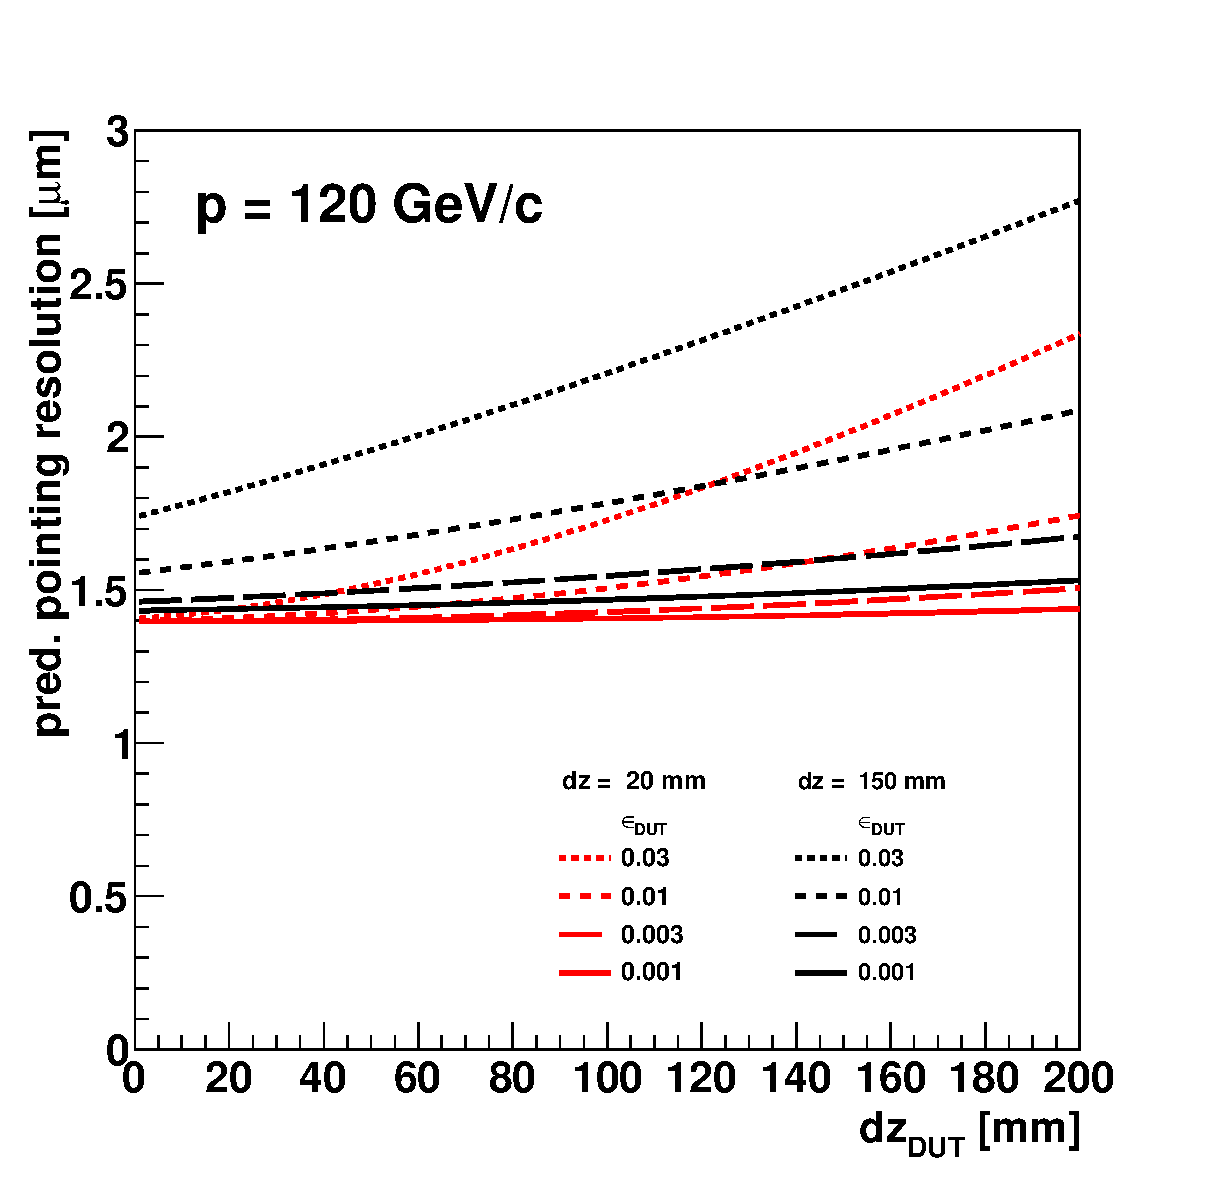
\includegraphics[width=0.49\textwidth]{figures/CalcResoVsDzdut_Cern_2}\\
  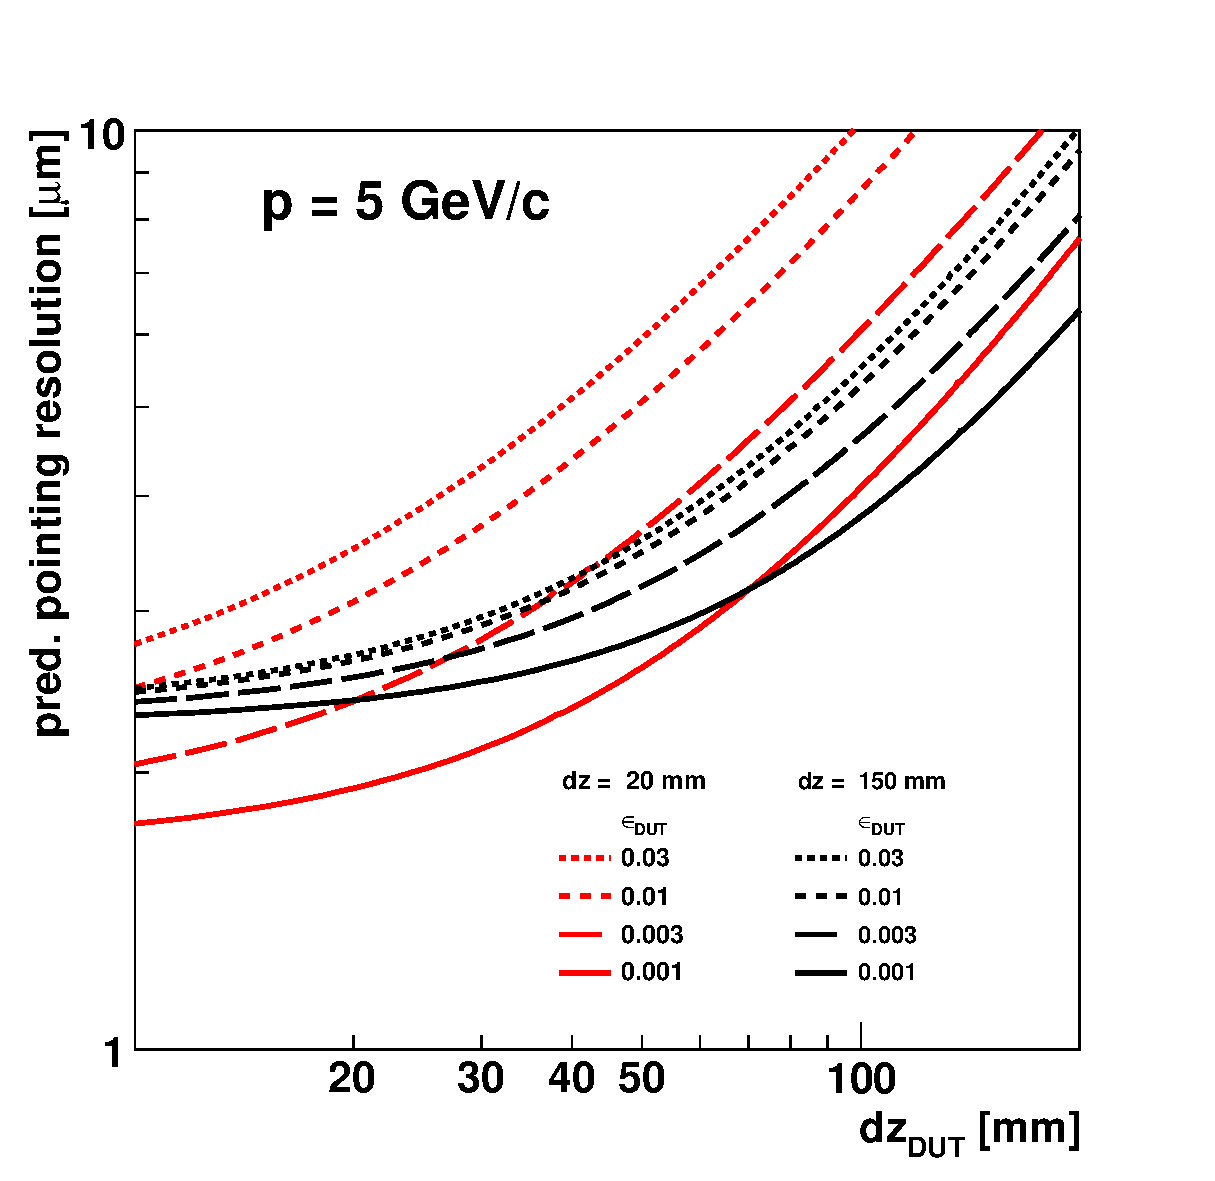
\includegraphics[width=0.49\textwidth]{figures/CalcResoVsDzdut_Desy_loglog_2}
  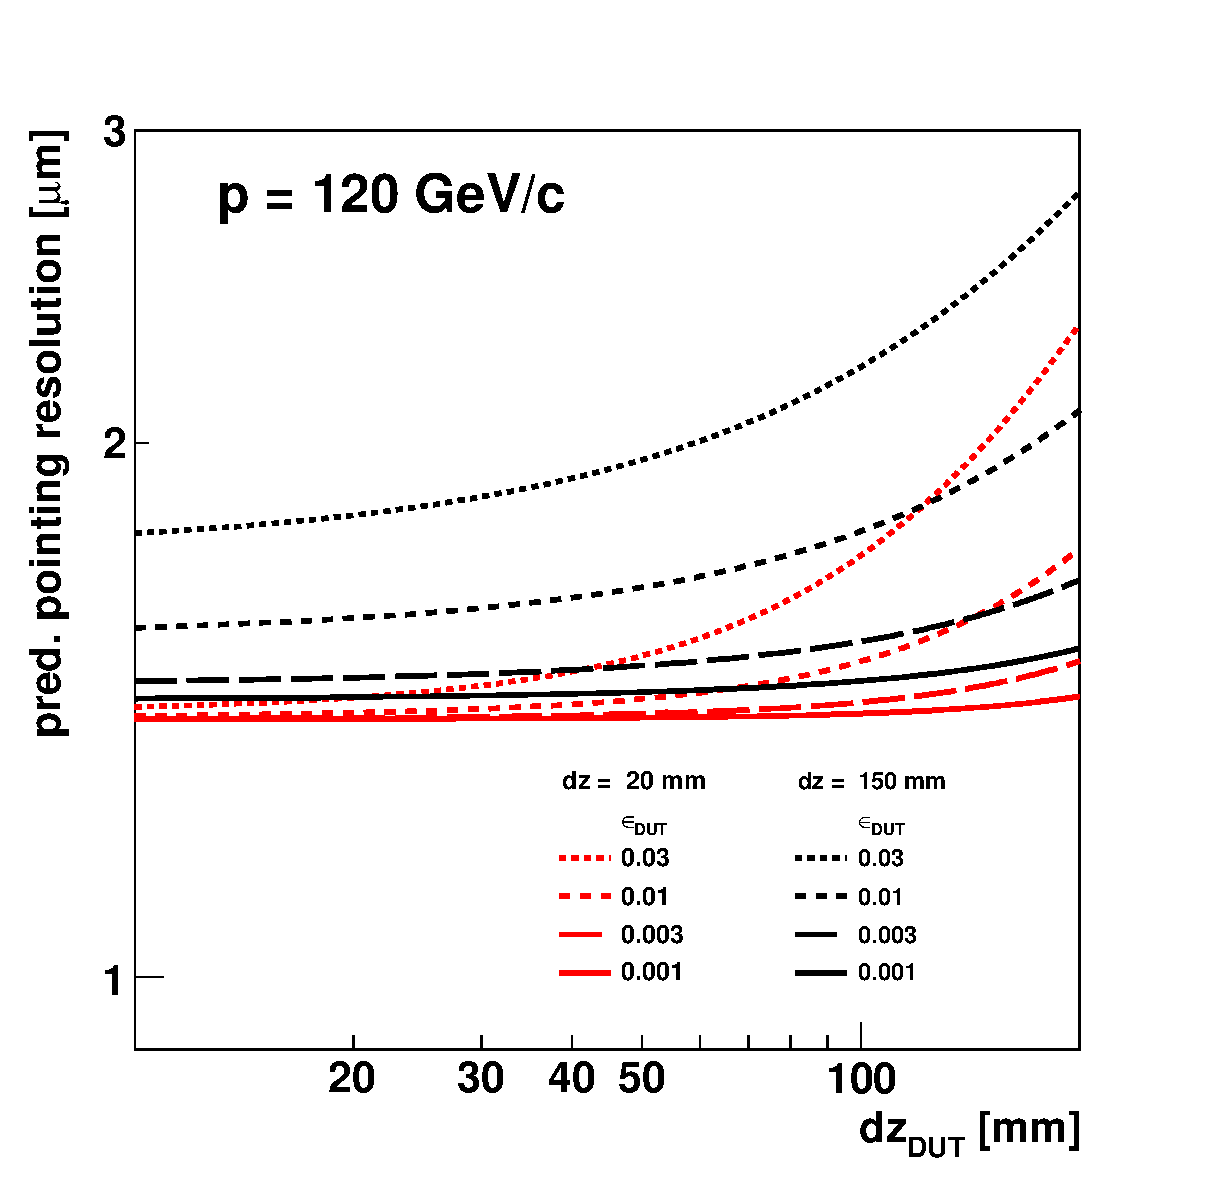
\includegraphics[width=0.49\textwidth]{figures/CalcResoVsDzdut_Cern_loglog_2}
  \caption[Pointing resolution for various DUTs as a function of the distance between DUT and neighbouring planes]{
  The pointing resolution for various DUTs is shown as a function of the equidistant distance between DUT and neighbouring planes.
  Left: at 5\,GeV, Right: at 120\,GeV. }
\label{fig:CalcResos_dzdut}
\end{figure}

A comparison between the measured resolution at the DUT with the calculated pointing resolution $\sigmapGBL$ is only possible, if the measured resolution is corrected by the DUT's resolution

\begin{equation}
 \sigmap = \sqrt{\sigmames^2 - \sigmadut^2}.
 \label{eq:sigmap}
\end{equation}

\noindent
This is shown in figure~\ref{fig:CalcResoP_DUT} (A) as a function of the beam momentum. 
Here, the pointing resolution is analytically calculated for a ``five planes plus DUT'' configuration, where the DUT is a $\Mimosa$ sensor, in order to match the measurements undertaken. 
The solid lines represent GBL calculations, the crosses are the $\sigmap$ corresponding to equation~(\ref{eq:sigmap}). 
The band formed by the solid lines represent the calculated pointing resolution assuming $\sigmai = (3.42 \pm 0.10)\,\upmu\meter$ for the wide and the narrow configuration. 
A nice agreement between the GBL calculations and the pointing resolution derived from the measured resolution is found.
In figure~\ref{fig:CalcResoP_DUT} (B) the achievable pointing resolution as a function of the material budget is plotted from a user's point of view, i.e.~for a ``six planes plus DUT'' configuration. 
Again it can be seen, that a minimal $\dzdut$ allows for the best possible resolution. 
The intersection for equally coloured lines mark the amount of material budget, where a change in the optimal plane spacing $\dz$ happens.
For budgets below (above) the intersection, a narrow (wide) configuration is preferred.
The position of the intersection shifts to smaller material budgets with increasing $\dzdut$. 

\begin{figure}[tbp]
  \centering
  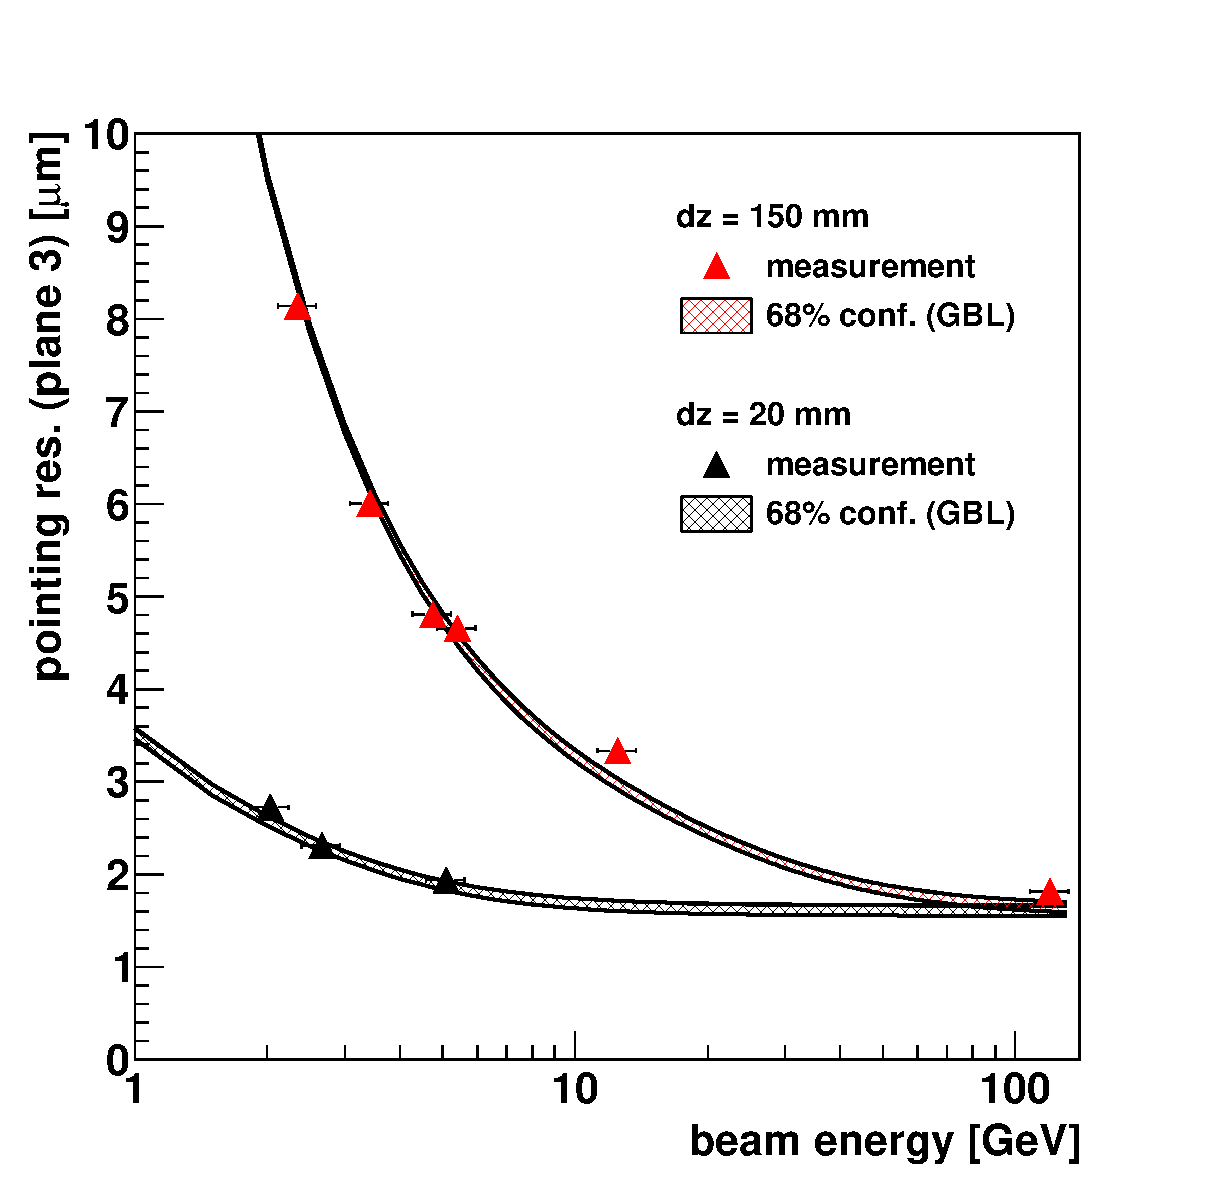
\includegraphics[width=0.49\textwidth]{figures/energy_plot}     \put(-125,175){(A)} % was CalcResoVsP
  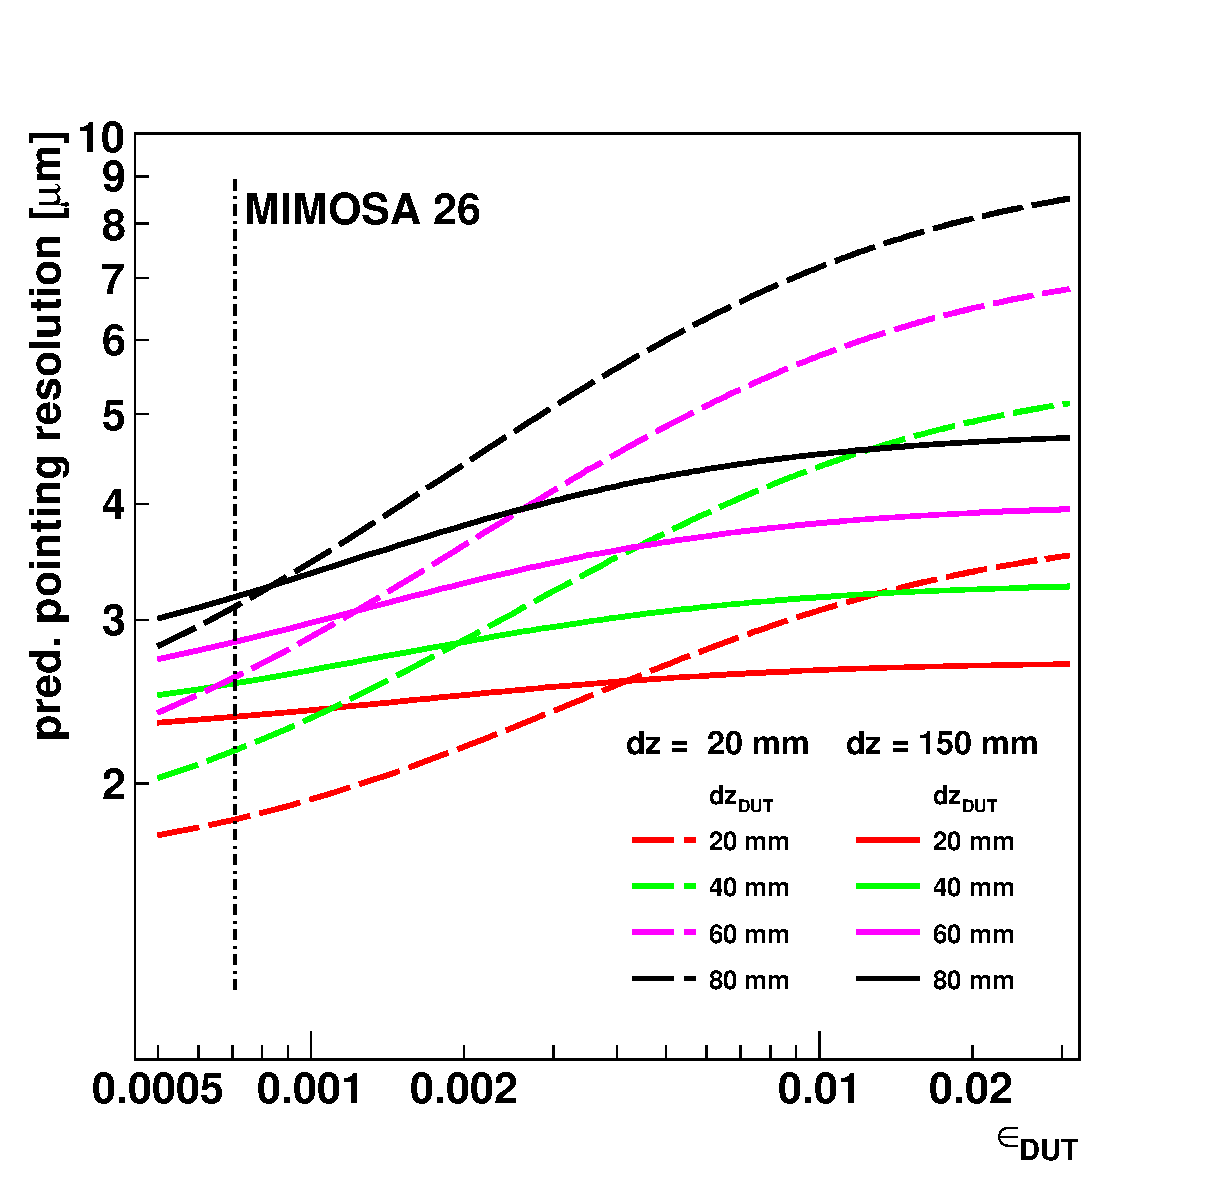
\includegraphics[width=0.49\textwidth]{figures/CalcResoVsEpsdut}\put(-125,175){(B)}
  \caption[Pointing resolution as a function of the beam energy]{
  (A) The pointing resolution for the wide (red) and the narrow (black) set-up is shown as a function of the beam energy for a 5-plane set-up for comparison with data. 
  The theoretical limit of about $1.6\,\upmu\meter$ for plane\,3 is indicated as a dashed line.
  Pointing resolutions derived from the measured resolutions at plane 3 for various energies and plane spacings are shown as crosses.
  (B) The pointing resolution for various geometries is shown as a function of $\epsdut$ for a 6-plane set-up.}
\label{fig:CalcResoP_DUT}
\end{figure}

Take note, that if straight line fitting is used, the inclusion of downstream planes might significantly deteriorate the unbiased residual widths,
 as kinks at the possibly thick DUT (and also the $\Mimosa$ planes themselves) are not allowed for in the fit.
Therefore, using GBL is always recommended. 
If straight line fitting is used nonetheless, a fit using the upstream planes only might result in a better unbiased residual width, compared to a fit that includes the downstream planes.
However, in a narrow ``six planes plus DUT'' set-up using a 5\,GeV beam, the pointing resolution at the DUT using GBL is $1.83\,\upmu\meter$, compared to more than $3.88\,\upmu\meter$ using only the upstream planes.
N.B., that in the ``upstream only'' case, the optimal plane distance is the wide configuration.
A web tool is available with compatible results in comparison with the GBL calculations is available.\,\cite{webtool}


comment hj:\\
apply energy correction (Ref Summer Student 2013) , then re-do reso vs energy plot
